\chapter{Reducing Collection Bloat}

 Relationships in an
entity-relationship model are typically implemented in Java using the
standard library collection classes. While a simple 1:1 relationship can be
implemented with a single map, more complex 1:n, n:1, and m:n are usually 
implemented with collections inside other
collections, sometimes nested three or more levels deep. 
As a result, it is common for a Java application to create hundreds of
thousands, even millions, of collections, where the vast majority have only a
very small number of entries.

Our guess is that the
collection class developers would be surprised by this usage pattern. 
Why would they have bothered implementing expandable
structures and clever hashing algorithms for only a few entries?
This mismatch between collection implementation and usage is 
a leading cause of memory bloat. The basic cost of a collection, even an
empty collection, is remarkably high. Creating millions of small collections
multiplies this basic infrastructure cost, which is all overhead, filling the
heap.
 
 This chapter shows
 how to mitigate the many-small-collections problem to reduce memory bloat.
 
 \section{Choosing The Right Collection}

There are many ways to implement a relationship. Conveniently, Java
collection classes make decisions easy: for a
set, use \class{HashSet}, for a map, use \class{HashMap}. 
If you need ordering, there are various lists; if you need sorted order, use
\class{TreeMap}. However, sometimes the obvious choice is more general than
necessary, and can lead to excessive memory bloat. 

To illustrate an overly general representation, consider a graph with 100,000
nodes that have four edges on average. 
An obvious implementation is to use a multi-valued \class{HashMap}, where the
 keys are nodes and the values are \class{HashSet}s of edges. 
 Figure\~ref{fig:graph-hashset} shows an entity-collection diagram for the
 graph.
 \begin{figure}
  \centering
 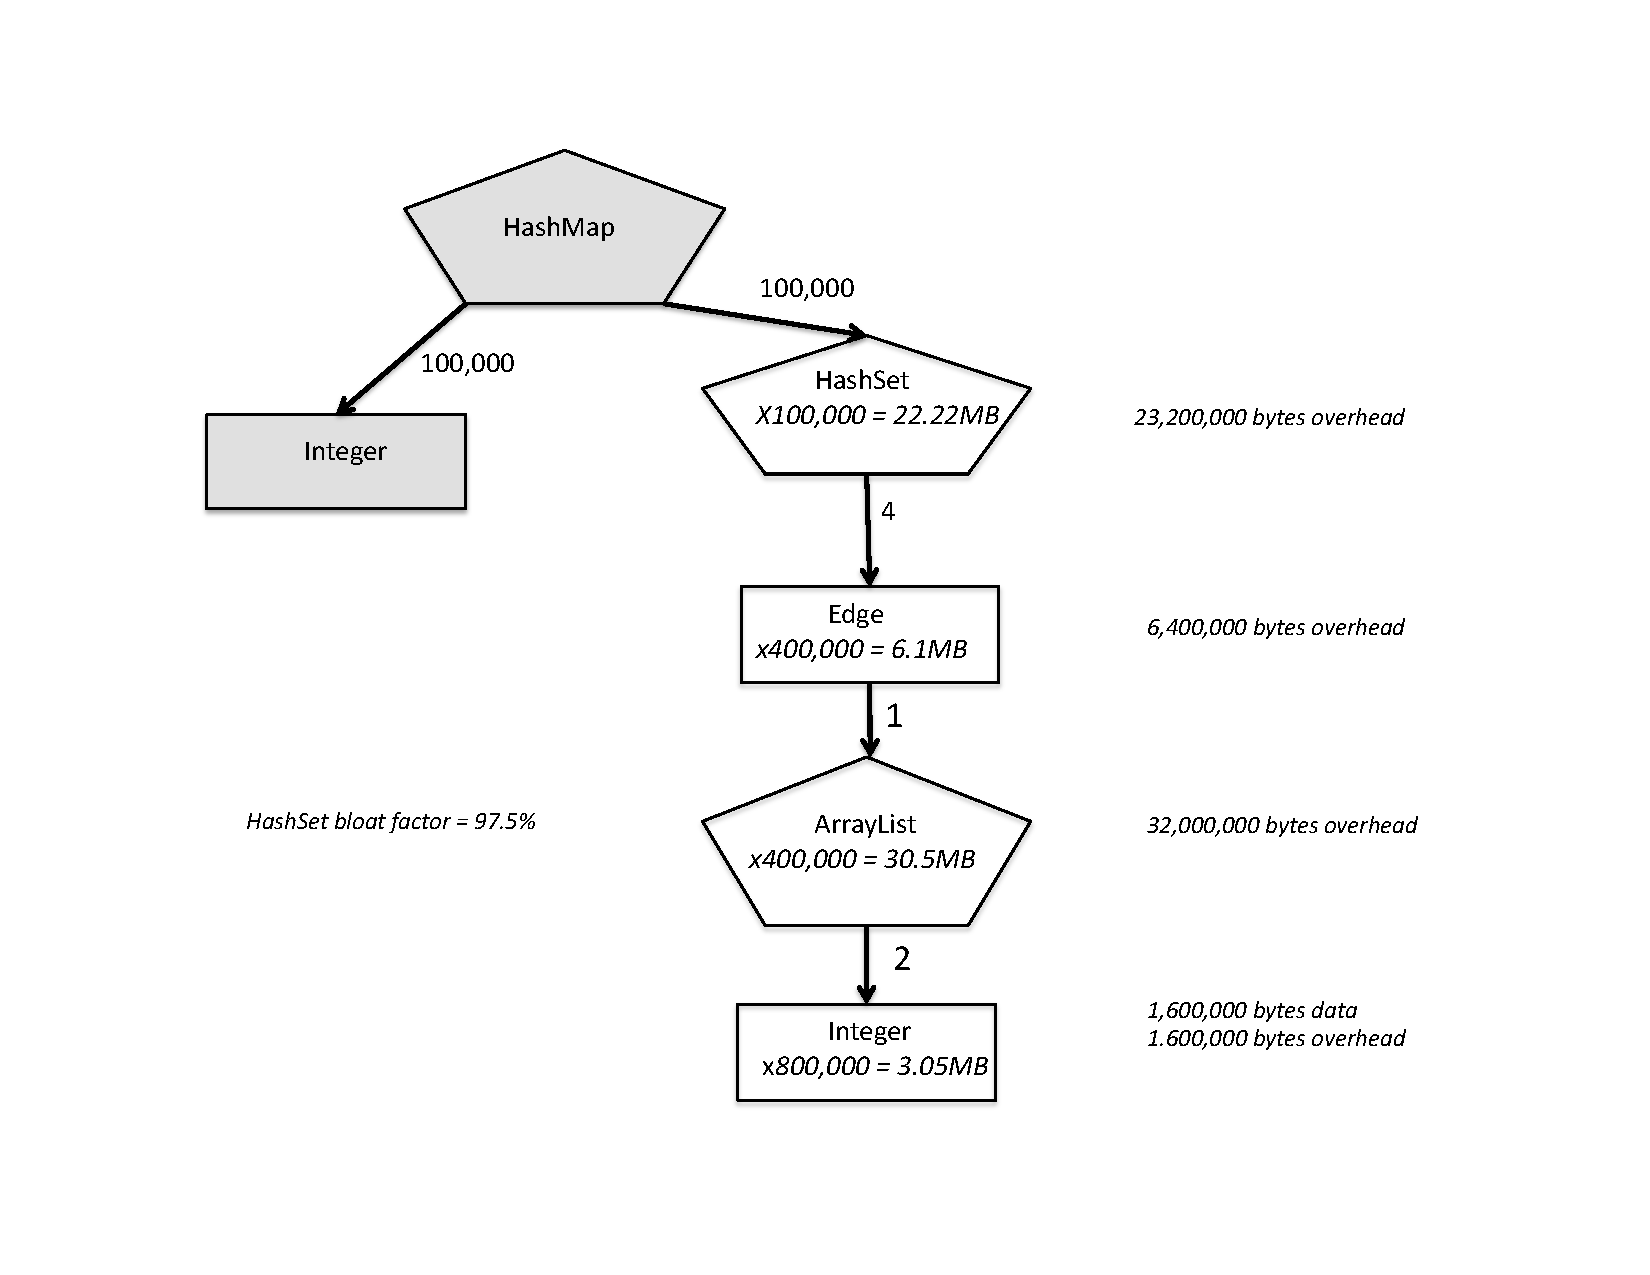
\includegraphics[width=.80\textwidth]{part3/Figures/graph-hashset.pdf}
  \caption{A 100,000 node graph, stored as a
  \class{HashMap} from \class{Nodes} to \class{HashSets} of \class{Edges}.}
  \label{fig:graph-hashset}
\end{figure}
%Sun library --  Empty HashSet -- 136 bytes
% 16 bytes HashSet (header + pointer)
% 40 byptes HashMap Object 
% 80 bytes empty array of entries

%HashMapEntry:  24 bytes:  header + 4 fields (value, key, next, hash)
% 4 entries -- 96 bytes
% total overhead for 4 entry hashset: 232 bytes
% 100,000 hashsets with 4 entries is 22.13MB

% HashMap size: 40 for header + 8 for array header
% 24 bytes per entry + 6 per entry in the array (assume extra for growth space)
% so for 100,000 entries, thats 48 + 3,000,000 bytes = 2.86MB
This example shows how easy it is to generate a lot of small collections with a very high overhead, 
in this case 100,000 four-element \class{HashSets} with a bloat factor of 89\%. Each \class{HashSet} 
by itself is 232 bytes of overhead, while four \class{Edges} have
contain only 32 bytes of data.

This implementation of a $1:n$ map is very common and
appears to be quite reasonable. However, when $n$ is small, 
the \class{HashSet} infrastructure overhead
overwhelms the data. Figure~\ref{fig:hashset} shows why a \class{HashSet}
has such a high overhead. Some of the
 overhead is Java-related, and cannot be avoided. Other overhead is the result
 of hard-coded assumptions about expected usage. The infrastructure is designed
 for fast access to a very large \class{HashSet}, with needs far different 
from one with a handful of entries.
 \begin{figure}
  \centering
 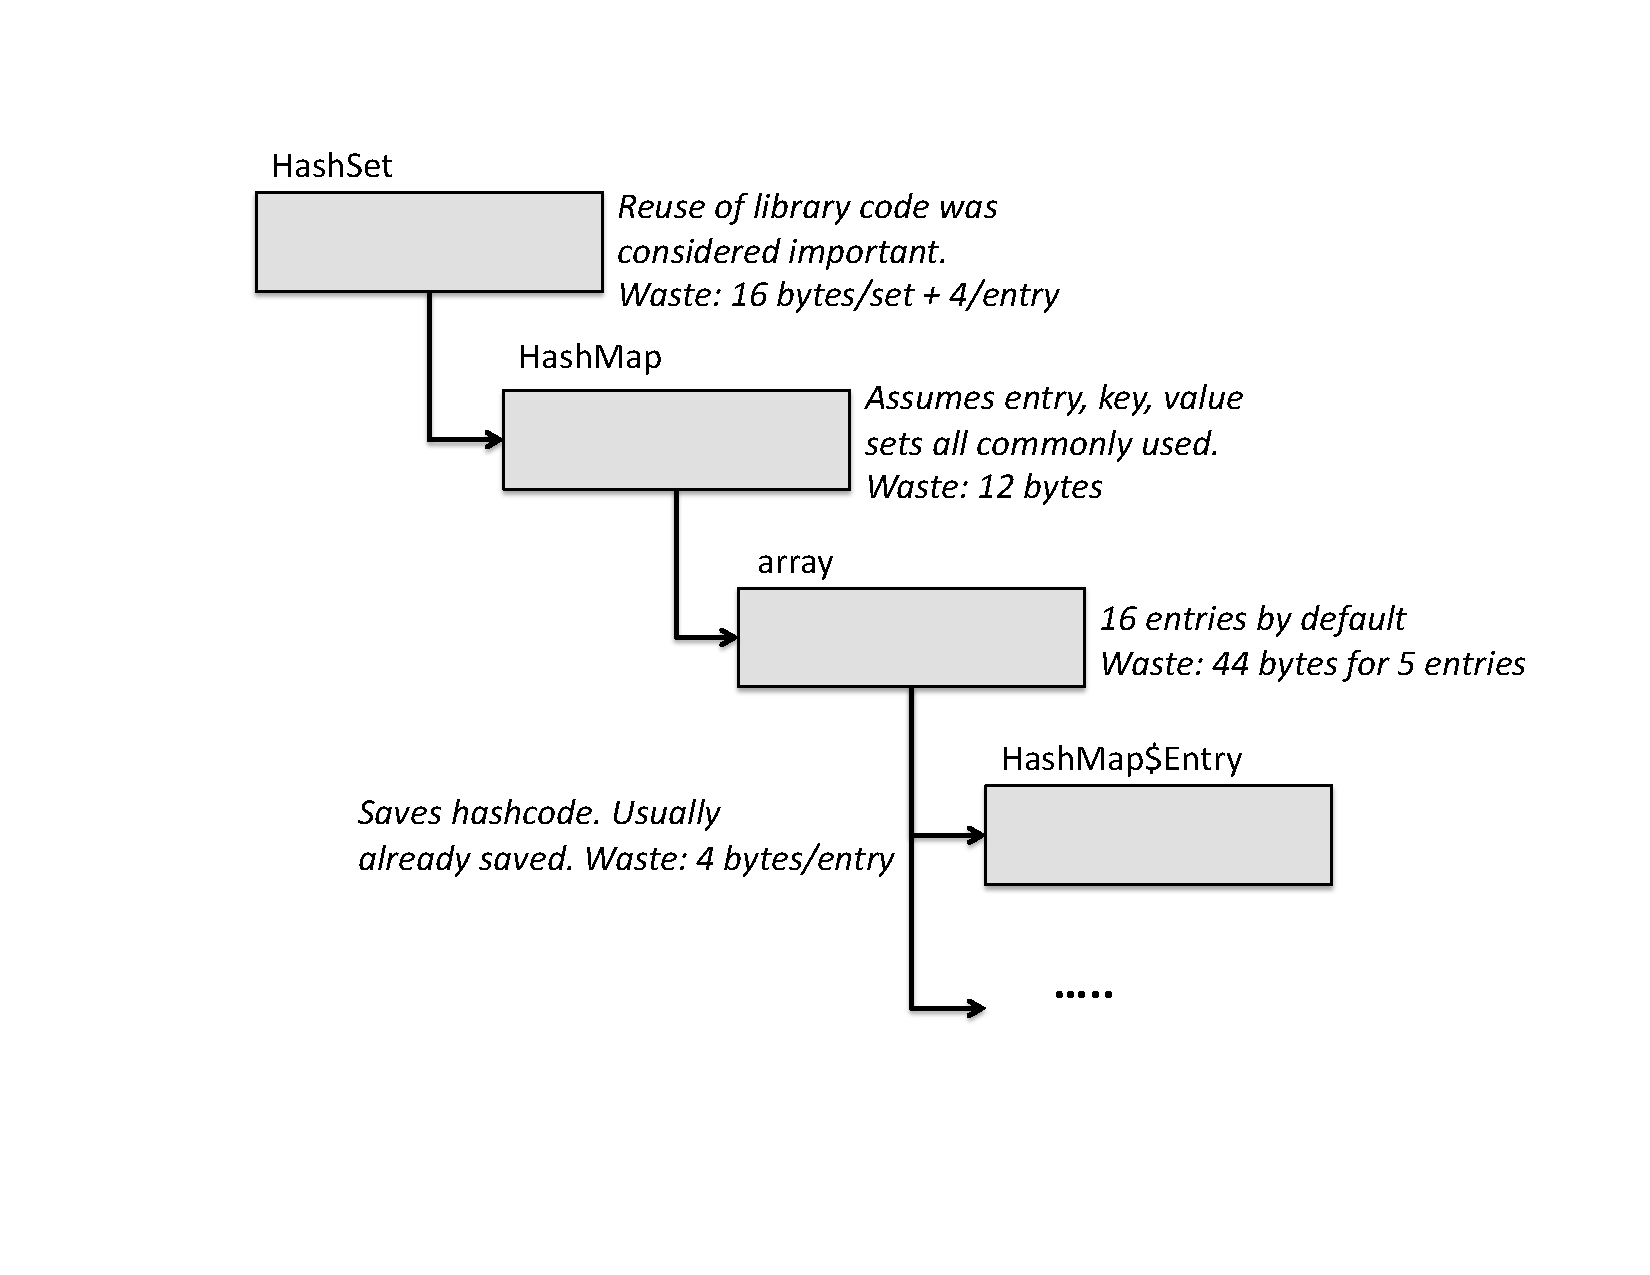
\includegraphics[width=.80\textwidth]{part3/Figures/hashset.pdf}
  \caption{The internal structure of a \class{HashSet} showing how
  implementation assumptions waste memory.}
  \label{fig:hashset}
\end{figure}

\paragraph{Reusing HashMap} Internally, a \class{HashSet} is just a wrapper,
delegating all of its work to a \class{HashMap}.
This decision to reuse the \class{HashMap} code instead of specializing
\class{HashSet} costs an extra 16 bytes, which is reasonable if
\class{HashSets} are big and the fixed overhead costs are amortized away. 
Unfortunately, fixed cost is magnified when there are many
small \class{HashSets}. 
Also, \class{HashMap} is
more general than needed.
Each \class{HashMap\$Entry} stores a key and a
value, and \class{HashSet} only uses the key, so four bytes are wasted per
entry. Sometimes specialization is a better option than reuse, especially for
library classes, where the usage patterns are not known in advance.

  
\paragraph{Open Chaining} \class{HashMap} itself is fairly
 expensive. First, the \class{HashMap} object is just a container pointing
 to the actual array of entries. This delegation is necessary in Java.
 Secondly, \class{HashMap} uses an
 open chaining algorithm, which means that each entry requires its own
 \class{HashMap\$Entry} object,
 
   On top of  it, 
the default size of the array, if you don�t specify something is 16. 
 So you get 16 size array, and this is all fixed cost. Before we have even
gotten to the cost of the actual entries in it. 


 The third problem is that hashmap 
has a bunch of bookkeeping fields in it, that really are rarely needed, 
and certainly not needed all together. It has a bunch of fields to keep different 
views of the hashmap that you might want. The map interface says that you can 
compute a collection of all the entries, all the keys, and all the values.
 And HashMAp caches all of those. So every HashMap, and every HashSet, is paying these three 
 pointer costs, which is an extra 12 bytes. In fact, you rarely use all three together, and 
 it�s not all that common to use even one of them. 

The other thing is that the hashmap entry itself is storing a hashcode. 
It�s maintaining a hashcode, even though the most common cases are keys, 
either strings, store their own hashcode. Or integers, where the hashcode 
computation is pretty trivial. So that�s also a misplaced optimization, 
and you have to ask the question. Was this based on an empirical study, 
with possibly the wrong benchmarks, or was this based on some assumptions? 
In this case, it was sort of another cautionary tale for library designers of 
the danger of premature optimizations.

The end result is that HashSet is a pretty poor choice if you have small sets. 
 At least with its current implementation. Obviously, it�s worth measuring here. 
 And indeed the developer did, and was able to solve the problem. Some other 
 lessons in here about what the developers of hashset must have been thinking, 
 and really for anyone who is developing a library of framework that is going to 
 be used higher up. Basically, they hardcoded in a lot of the assumptions about 
 its expected usage.
 

\section{Transforming Fixed Size Collections}

Getting back to our example, the developer looked and said, I actually 
don�t need the hashset functionality, because the only difference in functionality 
between a hashset and an array list is that the hashset was guaranteeing 
uniqueness, and it turns out the developer was already guaranteeing uniqueness 
in the loading code, so this was just put in as an extra failsafe thing, just in 
case there was a bug in the higher level code. When the developer saw this, 
he said, that extra check is not worth the cost. Was able to replace this with an 
arraylist, and for this piece of the structure was able to get 77\% savings
pretty easily.  Obviously, if we could have collections that worried about all 
of this stuff for you. A set that grows more gracefully, that you didn�t have to 
pay a high fixed cost for a tiny little set, then it would be very nice.

L
\section{Properly Sizing Collections}

 Let�s talk a little bit about default sizes and growth policies, and that 
 sort of thing. So this is a little hypothetical experiment here. We�re getting 
 back to the value side of this structure, where you replace the original 
 hashsets by arraylist. He sized them minimally, but having not done that, 
 had he taken the default sizes for the arraylists, it would have cost another
 28\% of overhead, since all the collections, basically are sized pretty 
 aggressively just like StringBuffer is, with this idea of trying to reduce 
 the copying costs and basically assuming that any collections you have are 
 going to grow, and so we�d better pay those costs up front in large chunks, 
 so that you don�t have to constantly pay a reallocation, and copy costs, 
 and it�s really an open question of whether that�s buying us any performance 
 or not, it�s certainly costing people a lot of footprint. One of the common 
 patterns we see is people just take the default size of collections. 
 They just take the constructor, no parameters, and even when they do 
 specify a default size, the collection growth policies are still pretty 
 aggressive. Typically double in size, and there�s even one copy constructor 
 that one of the array list copy constructure, if you hand it a collection and 
 say make me an arraylist out of this, it actually adds 10\% to it, just in
 case you grow this thing. And the typical pattern is you are building some 
 temporary collection to sort something or filter something, and at the last 
 minute you are done with it, and you turn it into an arraylist that you are 
 going to send onto somebody else, and they are not going to modify it again. 
 So there is definitely optimization for some questionable cases in here.

What can you do about this? One is that you can set the initial capacity 
relatively low. If you might be introducing a performance problem then do 
some timing, and see if it�s actually the case. Another thing is if you have 
data modes and many data models have this pattern, where you have a load phase 
vs a usage phase. I load all my data, and I never modify it again. Or maybe 
I�m modifying entries but never adding anything , then you can use  trimToSize. 
Just walk through the whole data model and call trimToSize on every collection. 
You will pay a reallocation and copying cost just once, and that�s it. 


Just a quick look at some of the default sizes. LinkedList, 
it�s not really applicable other than the fact � always comes with an 
extra entry as a sentinel, just to make the coding of LinkedList simpler, 
So you are actually paying 3 entry cost for a 2 element collection. 
ArrayLists, the default size is 10. For some reason, the latest J9, 
in these Harmony classes, which are open source, they�ve upped it to 12, 
and I�m not quite sure why they�ve done that. Actually that�s not really true.
 The default size initially for an empty collection is 0, so they�re still
 allocating the array with 0 size. Where as the Sun and older JVM�s are always 
 allocating 10 element collection. But on the Harmony classes, the new J9, 
 after you add the first element, they jump it to 12. It�s pretty hard not to 
 get those big jumps in these collection classes. HashMap, the default is 16, 
 and HashSet as well, since it�s based on HashMap. So it�s definitely 
 worth setting the default in these cases where you know you have mostly these 
 small collections. 

\section{Avoiding Empty Collections}

A related problem is empty collections, and this is super, super common. 
People are eagerly initializing things, and without realizing that the empty 
collections are pretty costly too. This was the case from JPMorgan 
Chase critsit, that Nick did, and in fact in SessionState, which had all sorts 
of other stuff in it, had these profile objects in it, which were profiles of 
customers, and each of those profiles was a highly delegated design, we saw it 
last week, each one had 40 instances hidden inside that box. 

For those of you who weren�t here last week, this notation is kind of a UML-like 
notation This is a logical data structure and these boxes are hiding other classes.
 The octagonal shaped ones are collections, things implementing relationships. 
 SO profile had quite a few classes inside it, and they all had the same coding 
 pattern in them, where they had these arraylists hanging off of them. 
 In one case it was to track the history of modifications in various fields. 
 In total, each usersession data had 210 empty arraylists hanging off of it, 
 which was rather expensive in this little example here. They were paying  
 8MB in this of just empty arraylists. So what are the remedies here? 
 The simplest thing is to lazily allocate these things. Along with lazy 
 allocation, there�s a nice static method in the collections class, 
called emptyset, where it will return you a pointer to a singleton empty set 
that has all the functionality of a set. EmptySet, EmptyList, EmptyMap, and 
those are great since you can point to them, and the size method will still work,
iterators will still work, all that stuff will still work, and you don�t have 
to allocate an empty collection. The only bad thing with those 2 patterns, 
and you really have to watch out for, is if you give out any references to your 
collections before they�ve been allocated. Because once you give out a 
reference, you expect people to hold on to it, then there�s no way to morph it 
into this other form that�s actually populated. And that�s a serious issue in Java.
 But if you can hide the references within the class, then this is very easy 
 to fix. 

So just a quick look inside the empty collections, you can see that they are not 
all that empty. So all the standard Java collections eagerly allocate their 
subsidiary objects, which means that every empty collection consists of 2 objects, 
2 object headers, a pointer, plus whatever bookkeeping fields they have. 
So you get these rippling effects, you have a really high level code, that�s 
eagerly initializing some package, and it�s eagerly initializing some thing else,
 and eventually it�s initializing some collection, and the collection is doing 
 the same thing; it says, well I�m just going ahead and allocate my array, 
it�s not clear why, it�s either ease of coding, or to avoid an if statement 
check at runtime, it�s not clear. So another area is to see if there�s any 
 performance benefit to this, or is this something that can be changed very 
easily. And juust a quick look at the cost of the empty collections. 
What strikes me � these are the number from both sun and IBM. What strikes
me is that the smallest number here is 48, so there�s certainly no single 
digit anything in Java, but 48 is a pretty high number for something that�s 
empty, if you are going to have a lot of them, and also, there�s a little bit 
of variation, both having to do with whether you�ve made the size default or not, 
and also what kinds of collection class you are choosing.

